\section{System Overview}
\label{overview}
\noindent
Heimdall has two components: the first is an app installed on a user's mobile device and the second is a Web service that receives install, uninstall and update notifications when these events occur on the device. Upon notification, the server processes all heuristics that apply to the app and generates a set of actions for a system administrator. At this point the system administrator can take an appropriate action based on the detected threat level. Our present prototype, includes a simple content provider heuristic that estimates the impact of a vulnerability. The only solution that is possible, at the moment, is to uninstall the app and that notification is then sent back to the user's device automatically.

\begin{figure}[tb]
	\centering
	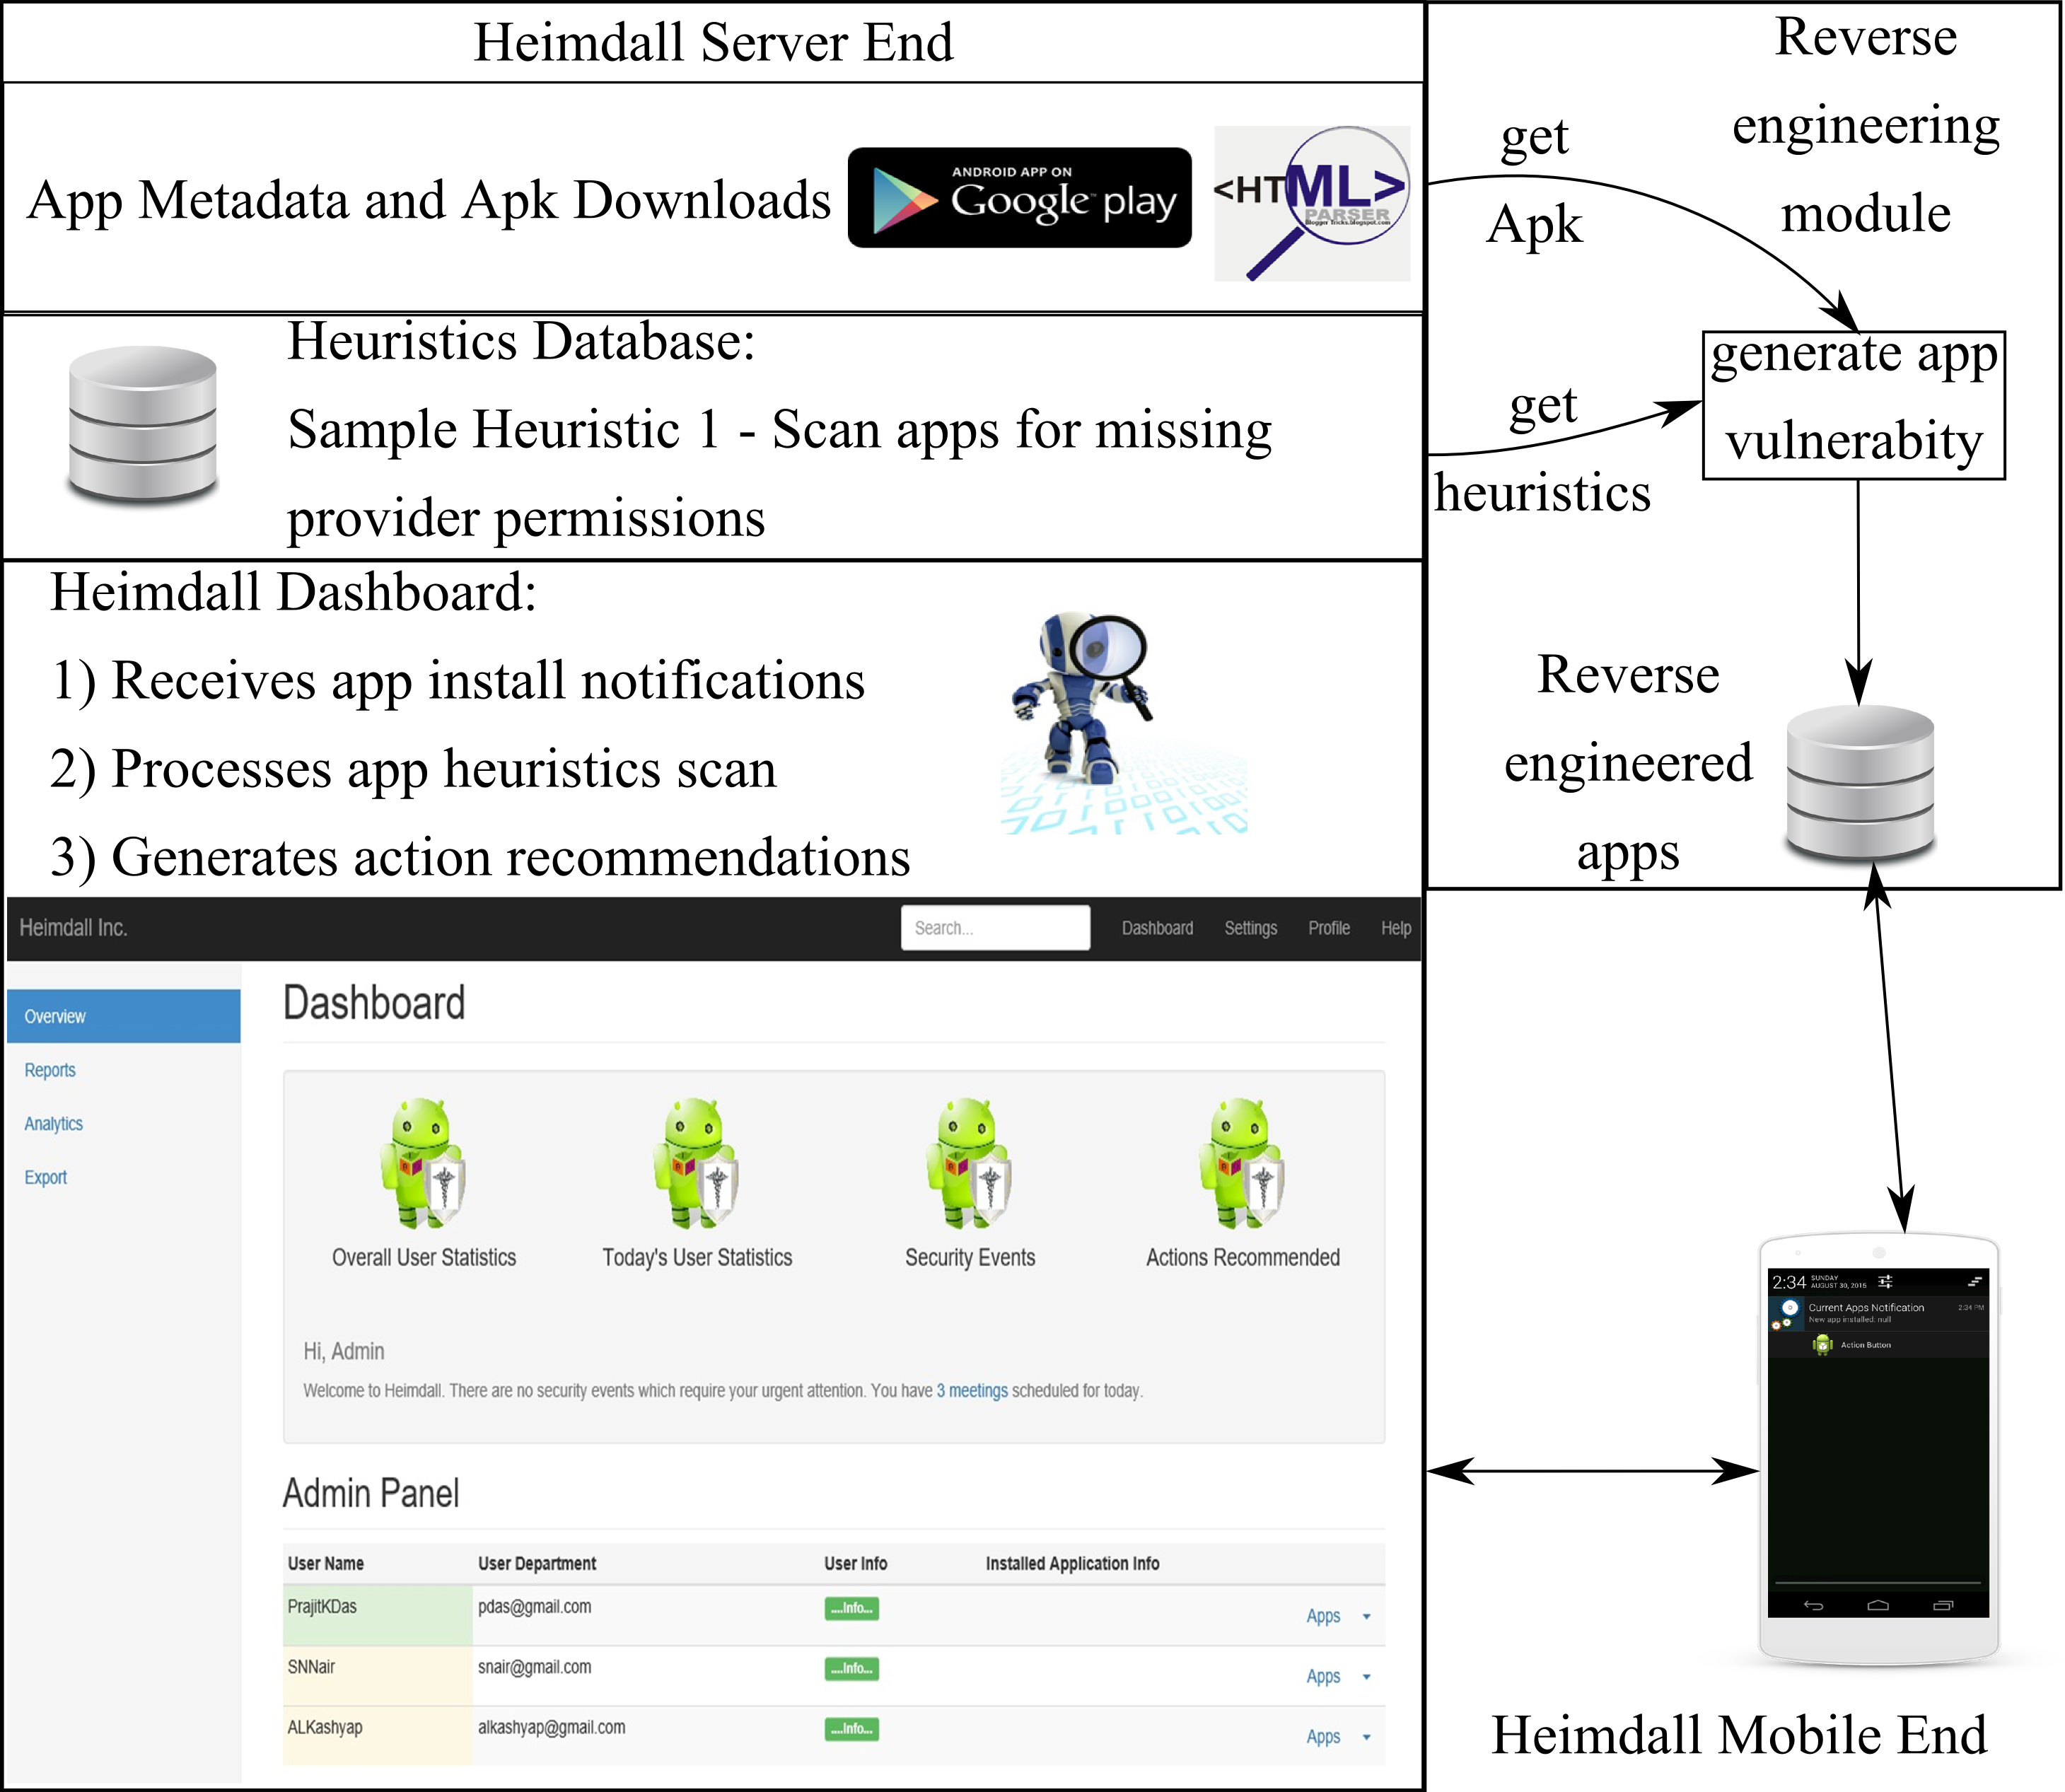
\includegraphics[width=\columnwidth]{images/architecture}
	\caption{System Overview}
	\label{fig:arch}
\end{figure}

Heimdall server has two additional capabilities. The first is to generate reverse engineered apps that we then test on the mobile devices. The reverse engineering process removes any provider associated permission and ensures that the ``exported'' tag for the provider is set to true. The second capability is to detect missing provider permissions for known apps. For demonstrating these capabilities, we downloaded about 1500 apps from the Google Play Store. We used a tool called apktool~\footnote{A tool for reverse engineering 3rd party, closed, binary Android apps~\url{https://ibotpeaches.github.io/Apktool/}} to decompile the Android binary application packages (apks) and parse the manifest files to detect the presence of such a vulnerability in the apps. Naturally, as we include more heuristics, Heimdall will become capable of detecting more such vulnerabilities.

%\begin{figure}[tb]
	%\centering
	%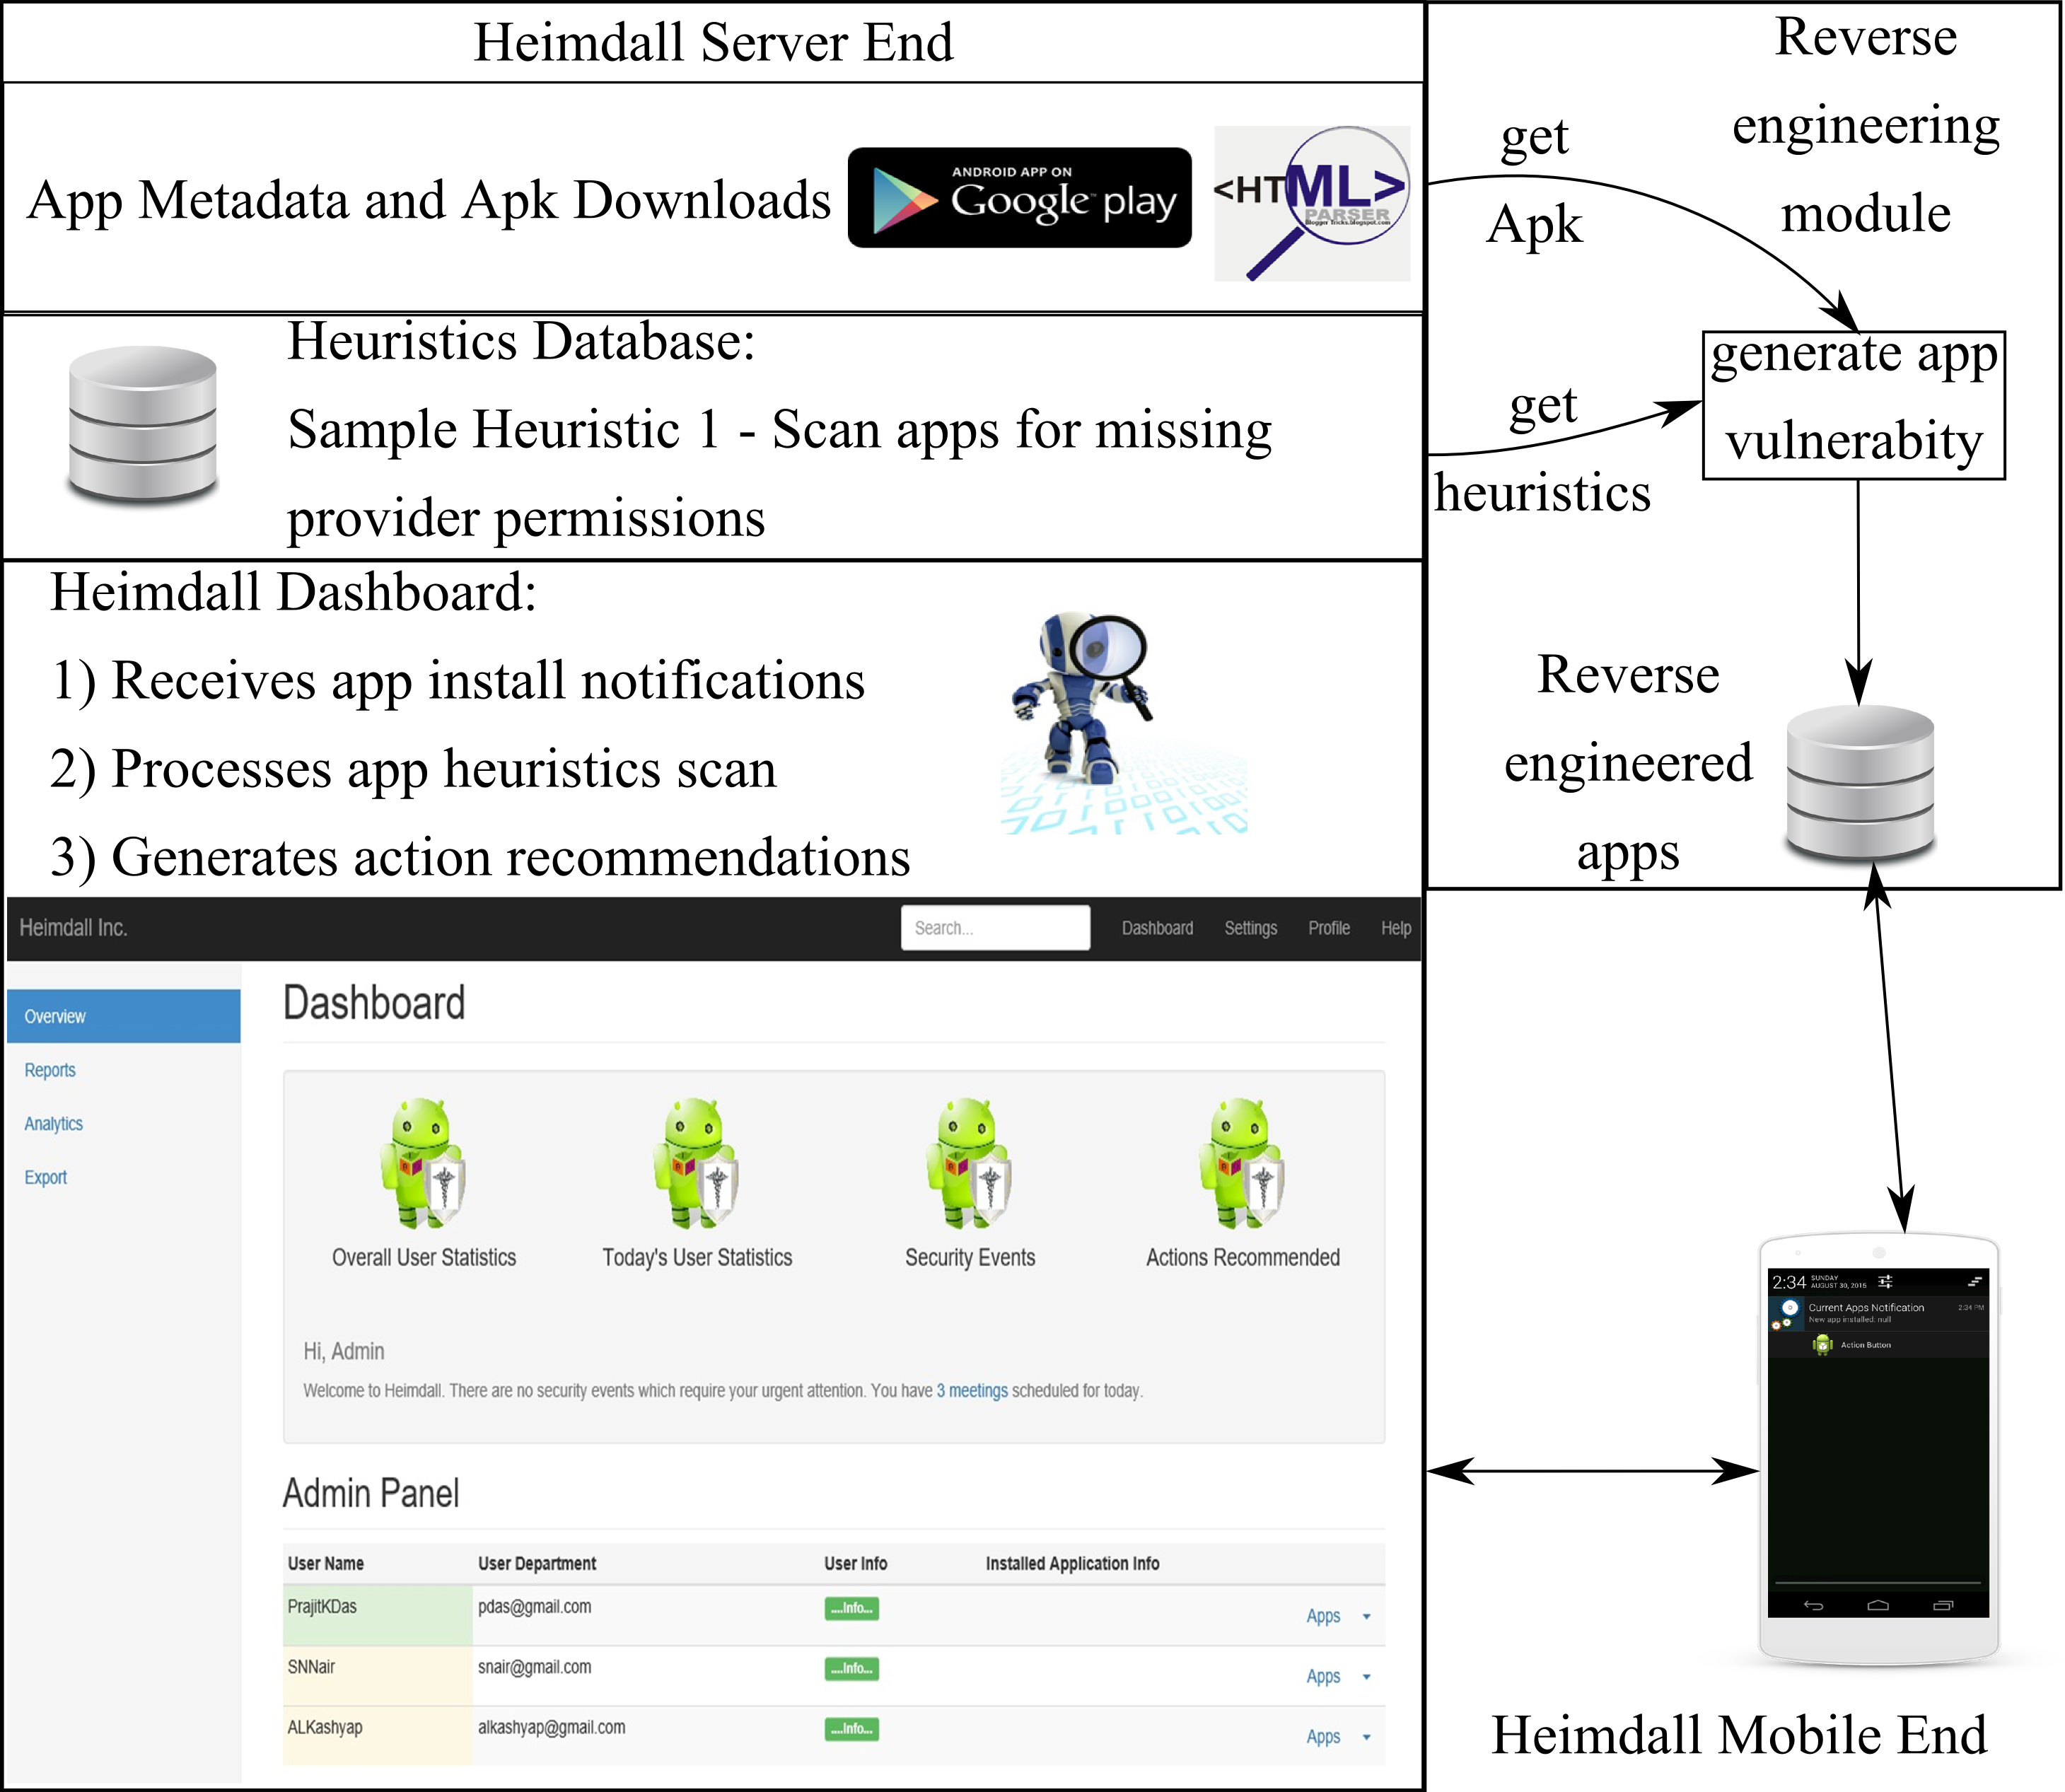
\includegraphics[width=\columnwidth]{images/architecture}
	%\caption{System Architecture}
	%\label{fig:arch}
%\end{figure}
